% !Mode:: "TeX:UTF-8"
% !TEX root = tjumain.tex

\iffalse
\bibliography{reference/reference.bib} % 欺骗latextools获取bib文件
\fi

%%%%%%% 正文 %%%%%%%

\chapter{绪论}

\section{研究背景及意义}

伴随着互联网多媒体技术飞速发展以及智能手机等终端设备的普及,同时因为各种短视频和社交软件的流行,全世界时时刻刻都会产生海量的图像等网络信息。在如今生活中,人们热衷于在微博、微信、Facebook、抖音等社交和短视频软件上通过图片、视频分享生活,图像作为传输信息的载体,包含了丰富的内容,如何从海量图像信息中获取有的人们所需要的信息变得越发困难,因此在计算机视觉领域中如何自动的对图像进行识别有着重要意义。于此同时,在我们现实中的图像信息内容更加复杂,很多时候都存在着大小、比例、遮挡等问题,这使得图像分类方式的研究更具有挑战性和现实意义。同样使得分类逐渐成为人工智能领域一个重要研究方向,并成为了机器学习和模式识别的基本问题。

现阶段机器学习算法大多是通过对已有的大量的数据的学习从而认识某种规律,且运用所认识的规律对未知数据进行预测,最终使计算机获得不断“学习”的能力。依据不同的学习方式可将机器学习分为监督学习、无监督学习、半监督学习以及增强学习。监督学习是利用已知类别的数据样本学习并且调整分类器模型参数,使其不管输入什么待测样本,其输出结果都能达到预期结果。监督学习的训练集要求包括输入和输出,即特征和目标。训练集中的目标一般是由人手工标注的。监督学习包括回归分析和统计分类两大基本任务。

分类任务指的是当且仅当预测样本的输出取值范围是有限个离散值,也就是说预测未知样本所属的类别属性。图像分类依据图像中目标所反映的不同特征,把这些目标区分开的方式。图像分类技术在现在的生活中有着普遍应用,例如支付宝以及各种支付软件人脸支付系统,智能手机解锁人脸识别系统,医疗领域中病变区域的识别,以及军事中地理信息的分辨等都是以图像分类技术为基础。

传统分类问题以怎样将待预测目标精准地划分到某一类中为探究目标.假如待预测的目标类别中仅仅包含一个或两个候选类, 那么这类问题被称作单分类或二值分类问题,也就是说预测该未知样本是否属于该类别。假如候选类别的数目有很多个,则需要在目标类别中选出一个候选类当作待预测样本的分类结果,那么这类问题就被称为多分类问题。传统分类问题注重的是将图像分类到某个单一的标签,也就是说仅对应唯一的语义信息,所以可以统称它们为单标签分类问题。与单标签分类相比较,因为客观物体本身的复杂性以及多义性,在实际应用中,一个对象同时属于多个类别是普遍存在的,就好比一本书既可以称做“作品”,又可以称它为“纸质出版物”,还可以依据其内容把它分为“经济”、“体育”等读物;可能会有与“金融”、“互联网”、“经济政策”同时有关的一段文本。所以为了能更好的表现出真实目标对象所具有的多语义性,常常用一个合适的标记子集来描述这个对象,多标记分类问题就这样形成了。每个样本都与一个由多个标记构成的相关标记子集合相对应,学习就是以未知样本预测其相应的标记子集为目标。

很显然,多标记分类问题更加符合真实世界客观对象的特性以及规律,但是解决多标记分类问题要面临许多的困难以及挑战。过于庞大的预测输出空间是最主要的困难。因为在多标记分类问题中,预测未知样本所对应的标记子集是我们需要做的,可是伴随着可以利用标记的数量增加,预测过程中所对应的候选标记子集的数量呈现指数型的增涨。毫无疑问想要从这指数级数量的候选子集空间中,选出正确的标签子集当作预测结果是一个巨大的挑战。因此有效减小标记输出空间成为解决多标记学习问题的一个重要策略。其中具有代表性的解决方案是基于地标标记选择和全标记恢复,这种方案通过选择关键的、具有代表性的地标标记和充分利用标记之间的相关性来实现对所有标记的恢复。随着现实世界客观对象变得愈发多义性,多标记分类面临更大的预测输出空间,研究如何有效减小标记输出空间和探索基于地标引导从而恢复所有标记就变得十分必要。

多标记分类问题面临的另一个难点在于如何有效地对单个输入和多个目标类进行建模,而传统的多分类问题只需要对单输入和单目标建立准确的对应关系。这种一对多的特性进一步增加了多标记模型预测所有可能标记的难度。因此准确而显式地对输入样本和多个目标类进行建模也成为解决多标记分类问题的一个重要方向。基于地标选择和全标记恢复的策略主要关注一些关键标记的特性和利用标记之间的相关性,进一步地有研究表明每个类标记都应该具有自己的特定特征,这意味着我们可以拓展关键标记的特性到所有类标记特定的特征学习。随着近些年深度学习\cite{Read2011Classifier} 的快速发展,更多的传统机器学习算法被扩展到深度神经网络框架中并借助其高度抽象的特征表达能力来获得性能的提升。因此基于深度学习框架下去探索全部标记特定的特征学习就变得非常有意义。

\section{国内外研究现状及存在的问题}
经历了数十年的技术沉淀,多标签分类技术得到了广泛的发展,非常多的对标签图像分类技术被研究人员相继提出,现如今在,多标签图像分类方法整体可被看作传统的多标签分类方式即基于词袋模型(BoW)方法和基于深度学习的方法。

\subsection{传统多标记分类的研究现状及存在的问题}
多标记学习是利用己有的训练数据学习一个模型,该模型可以为一个测试实例分配多个标记。多标记学习算法主要分为两类:问题转换和算法适应。转化基本问题的方法通常是将多标记问题转化成多个单标记问题进行研究。早期代表性的方法有Binary Relevance (BR)、Classifier Chains (CC) \cite{Read2011Classifier}、Label Pairwise (LP)\cite{Tsoumakas2007Random}等。基于算法自适应的方法是将已有的分类算法应用到多标记领域来求解多标记问题,典型的方法包括ML-KNN\cite{Zhang2007ML},ML-DT\cite{Clare2002Knowledge},Rank-SVM 等。此外,根据是否考虑标记之间的相关性还可以将多标记学习方法分为三种策略\cite{Agrawal2013Multi}:

a) “一阶策略”方法, 这类方法依次考虑每个标记并对其独立地进行处理,在这过程中并不考虑标签间的相关关系。代表算法有Binary Relevance (BR),
BR算法是将多标记问题当做多个单标记问题,然后分别给每一个标记训练一个分类器。这种方法思想简单,容易实现,但是因为没有考虑到标记之间的相关性,泛化能力不佳。其他“一阶策略”方法还有有:ML-kNN、ML-DT等。b) “二阶策略”方法,这种方法考虑的则是成对标记中两两之间的相关性,比如,样本所对应的相关标记与无关标记之间的排序关系或者每两个标记间的相互依赖影响等。虽然这种方法在一定程度上利用了标记相关性并且得到不错的泛化性能,但是如果实际应用中标记间存在的相关关系超过了这种二阶相关性,则分类性能会受到影响。代表算法有CLR\cite{Agrawal2013Multi}、LP算法等,其中CLR算法为两两标记重新构建数据集,将问题看做关于这个新建数据集的二分类问题,训练二分类模型,之后引入了人工分割点,将相关标记和不相关标记分隔开,再通过投票的方式比较人工分割点的票数和对应标记的票数确定一个实例是否含有该标记。此外,“二阶策略”方法还包括PS\cite{F2008Multilabel}、Rank-SVM等。c) “高阶策略”方法,这种方法在建立分类模型时往往要考虑每个标签以及其他所有标签之间存在的高阶相关关系。很显然这种方法较前两类方法来说对于真实世界中的复杂标签相关性拥有更强的建模能力,但是同时也有使得模型过于复杂的可能,从而导致大规模数据问题很难处理。典型算法有RAkEL\cite{Ge2018Multi}、ECC、EPS\cite{Read2008Multi}等,其中RAkEL通过从标记空间中随机选择k个标记作为新的标记空间训练一个分类器,该过程重复多次得到多个分类器,在测试阶段将所有分类器的输出结果做集成得到最终的结果。

上述方法主要是考虑如何有效捕获标记之间的相关性,为了进一步减小标记空间,一些学者提出基于地标选择的方法,这种方法首先在标记空间中选择一个小的标记集合作为地标性标记,这些地标性标记在标记空间中通常具有代表性,并且能和其他标记建立内部依赖关系。MOPLMS应用组稀疏学习策略去选择少量的标记作为地标标记,这些地标标记能重构出其他标记。ML-CSSP基于随机采样来进行地标选择,这里的每个类标记的采样概率反应了它在所有类标记中的重要性。尽管这些方法在一定程度上减小了标记空间,然而,这些方法将地标选择和地标预测分成了两个独立的步骤,这样即使其他的标记能被地标标记很好地恢复出来,但是地标标记本身可能很难通过输入样本被准确预测出来。

除了考虑标记之间的相关性和减小标记空间,最近,一些工作\cite{Li2015Leveraging}旨在从特征空间也学习某种关系,然后将这种关系作用到标记空间从而使得标记空间更加丰富。RELIAB\cite{Li2015Leveraging}和MLFE这两种方法将特征空间中实例与实例之间的关系传递到标记空间中,认为在实例空间中相近的实例在标记空间中也是相似的。此外,Jian等人提出的MIFS\cite{Jiang2016CNN}方法不仅通过聚类的方式挖掘了标记之间的相关性,同时也利用了特征空间的相关性。


\subsection{深度多标记分类的研究现状及存在的问题}

传统的多标记分类方法通常利用手工提取好的特征,无法端到端地去训练和学习模型,随着深度学习在图像分类领域的快速发展,很多研究工作开始直接利用深度卷积网络对图像进行特征提取,并设计和构建端到端的可训练模型。Gong等人\cite{Gong2014Deep} 将深度神经网络和基于排序的学习策略集合起来去解决图像标注问题;Hu等人\cite{Hu2016Learning} 提出一种结构化的推理神经网络去迁移多标记预测到多个语义概念层上;Wang等人\cite{Jiang2016CNN}将多标记图像分类转换成一个序列预测问题,并且用循环神经网络去探索标记之间的语义依赖。

为了进一步提高对图像的表达能力,最近一些工作引入了注意力机制。Wang等人引入了一个空间转换层去定位特征映射中的重要区域;Guo等人提出了注意力一致性的假设并且设计了一个两分支的网络,用原始图像和转换后的图像作为输入。这些基于注意力机制的方法虽然在多标记分类任务上已经取得了不错的效果,然而,他们没有考虑到类标记和局部视觉区域的准确的对应关系。主要原因是基于注意力机制的方法往往只利用了较弱的监督信息,即:“一袋标记”对“整张图像”而不是“特定的标记”对“特定的图像区域”。

此外,图结构被广泛应用于建模标记依赖和捕获标记之间复杂的相关性。一些基于概率图模型的方法包括条件随机场\cite{Ghamrawi2005Collective},依赖网络\cite{Guo2011Multi}和共现矩阵\cite{Xue2011Correlative}。最近,Li等人\cite{Li2014Multi}在标记互信息矩阵上引入最大生成树算法去构建标记图;Li等人 使用图Lasso框架学习图像依赖的条件标记结构;Lee等人通过合并结构化的知识图来提出了一种新的标记信息传播机制;Chen等人\cite{Chen2019Multi}首次提出一个基于图卷积网络的模型去捕获标记之间的相关性,它应用图卷积网络去映射标记表达到内部依赖目标分类器,但是该模型的多标记预测是直接用学到的目标分类器和全局的图像特征之间的相关性得分来表达,没有有效利用图像的局部特征。

\section{研究内容}
本文介绍以及分析了图像分类,尤其是多标签图像分类在机器学习领域的相关技术与研究,重点是深度学习方面。主要从问题转化方法和算法适应两个方面介绍多标签分类算法。本文中对于多标签图像分类问题,我们介绍并实验一种基于图卷积神经网络端到端的模型,它拥有多不例网络以及全局先验网络,不仅可以有效提取以及利用全局图像先验,更能学习良好的局部图像特征,再将二者有机融合。其针对标签之间相关性的建模以及通过相关性提升多标签分类精度有很好的效果。

\section{文章结构}
本文分析和讨论了基于深度学习的图像多标签分类相关理论和关键方法。针对多标签分类方法目前仍旧存在的问题以及模型设计的不完善,基于原有的方法和模型,通过一定的改进和融合,提出两种基于标签关联的多标签图像分类方法,通过试验分析了方法的优势和不足之处并据此明确此以后研究的方向。
 
第1章为绪论。本章非常详细地介绍和分析了多标签图像分类的课题来源、课题的研究意义以及国内外发展现状,并且阐述了图像多标签分类技术在实际生活方面的研究价值,从整体上说明本文的结构。

第2章  在这一章中我们对传统图像分类、基于深度学习的图像分类方法、图像多标签分类基本理论等做了重点介绍。首先针对目前多标签分类技术和其在多标签图像分类中应用的部分常见方法进行了系统介绍,其次我也重点阐述了卷积神经网络和循环升神经网络这两种深度网络,以及深度学习在目前多标签图像分类中的应用。

第 3 章本章主要介绍了基于一种新的基于GCN的多标签图像识别模型ML-GCN,介绍了其设计思想、基本理论、以及组成部分。本章主要通过概述,GCN图卷积神经网络介绍,ML-GCN整体框架以及相关系数矩阵介绍四小节对ML-GCN模型相关理论做了全面的介绍。

第 4 章主要围绕实验展开,首先描述评估指标、数据集和实现细节。然后,我们报告在MS-COCO\cite{Jiang2016CNN}和VOC 2007\cite{Zhang2007ML}了两个多标签图像识别数据集的实验验证结果。最后通过消融实验进行验证和探究。
 
第 5 章为总结与展望。对本总体的研究现状做了总结,并且通过实验对比分析了目前部分方法中的优缺点。并且进一步提出自己的见解。
 
\chapter{理论与技术}
\section{基于问题转化的方式}
在现实生活中,通常人们解决复杂的问题习惯将其分解,由大化小。换句话说,就是运用分治思想,把我们要解决解决的问题分解成许多个子问题,使得问题更加容易解决。从根本上讲,其实我们研究多标签图像分类是单标签图像分类向真实世界的衍生。问题转化的多标签图像分类方法是——将多标签图像分类问题转换成一个或多个的单标签图像分类问题,再运用成熟的单标签图像分类方式解决上述问题。

这种“多”转“单”的方法有很多,例如对每一个实例确定或是随机分配的一个标签,抑或是只保留只有一个标签的训练样本,然后用传统的多分类方法去训练。这种方法实际上会导致训练样本损失,因此并不推荐使用。再者,我们还可以将训练样本按每个标签去构造一个训练集,每个样本属于或者不属于此标签,对每个标签单独训练一个分类器,最后将多个分类器的结果合成。还有将每一个多标签都单独的视为一个新标签,在一个更多的标签集上做多分类。而当多标签的样本比较少时,这种方法就会受限。除此之外,对每个有多个标签的样本,复制样本,每个样本具有不同的标签,加入训练集后再使用覆盖分类法。

\subsection{传统的问题转化方法}
单标签分类技术作为机器学习视觉领域的重点研究方向,已具备数十年的技术沉淀,所以现如今的图像分类技术已经具备了基本成熟的框架,特征提却和分类器的构建无论对于传统的图像分类框架还是基于深度学习的图像分类框架都是核心步骤。传统的方法多数采用了Bag-of-Word(BOW)模型处理图像分类问题,即人工设计特征提取方式,下面本文将介绍基本的早期基于问题转化方法。

二元关系法BR(Binary Relevance),一种经典的基于问题转化方法的算法, 其原理简单来讲就是运用一个个独立的单分类方式解决每个标签的预测, 同时每个标签需要被训练一个独立的分类器, 并且用全部的训练数据对每个分类器进行训练。

为了形象描述,用G表示全部标签的集合, $G=\{\lambda j|j=1, …, n\}$, 我们在这里的$\lambda j$看作$G$中的标签, 同时将$H$当作多标签数据的训练集, $H=\{ (X_i, Y_i) |i=1, …, m\}$,其第$i$个样本的特征向量用$X_i$来表示,$Y_i (Y_i\in L) $被我们看作第$i$个样本所属的标签集合,如表1提供了一个多标签数据集的例子。

\begin{figure}[htbp!]
	\centering
	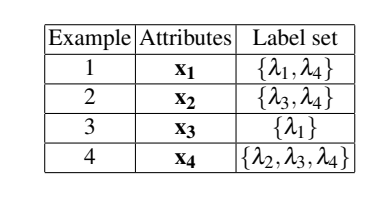
\includegraphics[width=0.75\textwidth]{figures/p2-1.png}
	\caption{多标签数据集例子}\label{fig:p2-1}
	\vspace{-1em}
\end{figure}

通过BR方法,这里每一个标签λj都将产生其自己单独的数据集,并且每个数据集包含训练集中的全部样本, 从而我们会得到N个数据集$H\lambda j (j=1…n)$,在$H\lambda j$中,所有数据集中所包含的样本都会被标注出是否属于$\lambda j$。BR算法的核心就是通过这个数据集训练得到一个二分类器$\lambda j$,并且其输出样本仅为是否属于$\lambda j$,进一步我们为每一个标签训练一个这样的二分类器。最后对于一个未知类别样本, 将全部二分类器结果组合在一起即得到了该样本最终的标签分类结果。表2显示的是将BR方法将表1转化的结果。

\begin{figure}[htbp!]
	\centering
	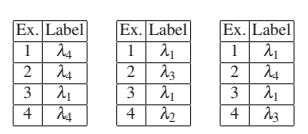
\includegraphics[width=0.75\textwidth]{figures/p2-2.png}
	\caption{BR转换的结果}\label{fig:p2-2}
	\vspace{-1em}
\end{figure}

通过原理分析我们很容易可以发现这种算法并没有考虑标签之间的相互关系,甚至将其直接忽略,所以其分类效果很难达到人们理想状态,基于此在文献\cite{Clare2002Knowledge}作者运用拷贝 (copy) 和带权重拷贝 (copy-weight) 的方法对BR进行了改进,将多标签数据拆分成多条单标签数据, 并给予相应的权重。如图3所示,表示表1通过改进BR改进算法转得到的结果结果,a)为拷贝 (copy)方法,b)为(copy-weight) 的方法。

\begin{figure}[htbp!]
	\centering
	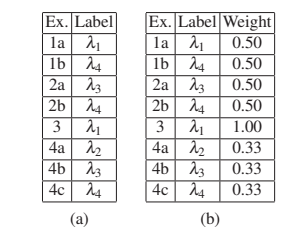
\includegraphics[width=0.75\textwidth]{figures/p2-3.png}
	\caption{BR改进转换结果}\label{fig:p2-3}
	\vspace{-1em}
\end{figure}

组合分类器链ECC (Ensembles of Classifier Chains)是另一种对于BR方法的一种改进, 通过上述阐释我们发现基本的BR算直接忽略签之间的相关性,这直接导致一定程度上的信息损失, 所考虑采用CC 分类器链,该方法可以在保持可接受的计算复杂度的同时对标签相关性进行建模。而作为BR的改进算法,ECC其主要思想便是用一条链将BR产生的N个二分类器链接起来,将训练样本经过每个二分类器的输出结果在加入到下一个而分类器的输入样本中进行训练, 换句话说就将其预测结果添至样本中, 继续代入下一个二分类器中训练。下面我们进一步通过举例说明,例如图3中的数据集中,我们以X为输入空间,Y为标签。

\begin{figure}[htbp!]
	\centering
	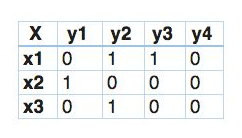
\includegraphics[width=0.75\textwidth]{figures/p2-4.png}
	\caption{一个多标签数据集}\label{fig:p2-4}
	\vspace{-1em}
\end{figure}

假设我们CC链含有四个二分类器,那么我们可以用图四形象刻画训练过程,如图四所示,我们用黄色部分表示输入样本空间,用白色部分表示每个二分类器的输出目标变量。

\begin{figure}[htbp!]
	\centering
	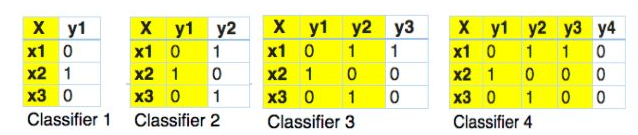
\includegraphics[width=0.75\textwidth]{figures/p2-5.png}
	\caption{ECC转换结果}\label{fig:p2-5}
	\vspace{-1em}
\end{figure}

通过对CC链基本理论分析我可以发现,在CC链中当二分类器排序顺序的不同时,其结果会有较大变化, 基于此ECC通常采用多条随机产生的不同标签序列的CC组合, 从而减轻单个CC由内部二分类器排列顺序问题而带来的不利影响。

标签幂集法LP (Label Powerset),被广同样也是一种使用广泛的的基于问题转化的方法。在LP算法中,我们考虑将训练数据中的每种标签集合进行二进制编码,然后使其形成新的单标签。因此研究人员将多标签数据以这种方式转化成单标签数据。原理如图5所示。

\begin{figure}[htbp!]
	\centering
	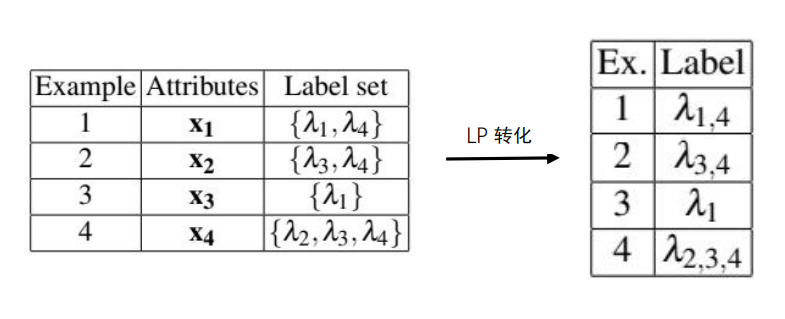
\includegraphics[width=0.75\textwidth]{figures/p2-6.png}
	\caption{LP转换结果}\label{fig:p2-6}
	\vspace{-1em}
\end{figure}

在LP算法的有一个显著缺点,就是其不能预测新的标签组合,.Read等人针对这一缺点创造性的将概率分布模型应用到LP中,是的其对未分类数据进行预测时, 可以预测出训练集合中未出现的标签组合\cite{Agrawal2013Multi}.如图6所示

\begin{figure}[htbp!]
	\centering
	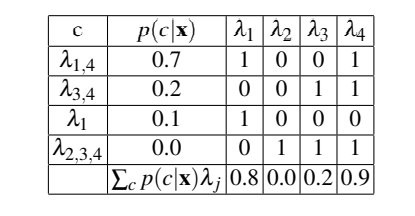
\includegraphics[width=0.75\textwidth]{figures/p2-7.png}
	\caption{LP概率分布方法}\label{fig:p2-7}
	\vspace{-1em}
\end{figure}

但是LP算法的复杂度较高, 达到$(min(2q, m)\times t(D))$ 。LP相对于$q$的计算复杂度取决于基分类器相对于类数的复杂度,等于训练集中不同的标签集的个数,这个数是最小值$(m,2q)$的上界,尽管如此它通常要小得多,但仍然会造成一个重要的复杂性问题,尤其是对于$m$和$q$值很大的情况。大量的类,其中许多与很少的示例相关联,这也使得学习过程非常困难。

\subsection{深度网络问题转换方法}

通常我们将深度学习理解为由许多非线性转换组成的体系结构,从而通过这种方式来抽象的表示输入对象。单标签图像数分类问题中深度卷积神经网络(CNN)取得了不同凡响的效果,因此得到了相关研究人员的普遍认可,从而使其近年来被广泛运用到多标签图像分类领域。

将深度卷积网络方法和SVM这一种传统的二分类器相结合,形成了CNN-SVM 模型。这种方法首先使用Image Net数据集预训练出来的卷积神经网络来提取待分类图像的语义特征,之后使用 SVM 方法对不同特征进行分类。由于SVM 是一种二分类器,无法直接进行多分类,基于此,CNN-SVM模型针对每一个类都分别构建了训练数据集,在针对每个类分别构建数据集的过程中将目标类的图像作为参考正样本,将其他全部的类别图像当作负样本而训练一个 SVM 分类器,在预测阶段中,将卷积网络中输出的所有图像语义特征逐次输入到各个 SVM 分类器中判断,以此得到图像中最终包含哪些具体目标。

除过利用多个SVM 分类器把多标签的图像分类问题转化为多个单标签的图像分类问题之外,通过图像分块且分别识别各图像块中的目标,是针对这种问题的另一种问题转换方式。其基本原理是通过相应算法将输入的图像合理分块,并使用CNN深度卷积神经网络为每一块图像分别预测其概率分布,最终的预测结果是利用融合算法将全部图像块融合得到的,其工作原理如图7所示。

\begin{figure}[htbp!]
	\centering
	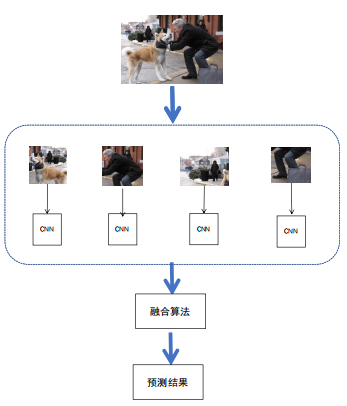
\includegraphics[width=7cm,height=10cm]{figures/p2-8.png}
	\caption{图分块识别框架模型}\label{fig:p2-8}
	\vspace{-1em}
\end{figure}

该方法中相应的图片分块算法多种多样,比如使用滑动窗口的方法将所输入的图像依次划分为大小不均一的数个图像块,然后通过计算各个图像块与训练集中图像的标注位置框的交并比,确定该图像块属于无关背景还是前景目标。在本文中使用的融合算法如下:
\begin{equation}
\label{dscNoStgProof0}
score(C_n) = \frac{1}{M}\sum_{i=1}^M y(C_n|P_i)^k
\end{equation}

其中$M$是该图像分块后图像块的数目,$y(C_n|P_i)^k$是图像块Pi中类Cn在神经网络中对应的输出值, $k$是大于1的常数。较高的$k$值会关注得分最高的图像块,相反弱化得分较低或适中的图像块的贡献。目标的大小、遮挡等一系列问题在多标签图像中比较常见,不同数据集图像的特征分布存在着较大差异,所以简单的采用滑动窗口实现分块的方式容易引起较多的无关背景,所以该方法不具备较好的鲁棒性。

\section{基于算法适应的方法}
目前,基于卷积神经网络的单标签图像分类算法已相对较为成熟。基于算法适应的方法的原理是利用特定的方式方法改造单标签的图像分类算法,以使其能够很好地用于解决多标签的图像分类问题中。能够用于改造的算法种类较多,例如通过相应方式改造boost kNN、SVM等算法以进行多分类。基于kNN算法的改造算法在实现多标签分类时能够加入先验概率,且能对输出的标签进行排序。基于SVM的多种改造算法中,有的研究者将L个二分类的算法训练结果加入到训练集中,之后再重复一次分类,不同的标签之间的依赖关系在这个方法中被考虑了进来,此法也是利用多个分类器进行叠加的一种特殊情况。还有的研究者在改造算法中采用了相关规则的挖掘方法。常用的改造方法主要分为两类,基于损失函数的改造方法和基于基础结构的改造方法,基于损失函数的方法通常根据对多标签图像分类的特性和特点设计了专用的损失函数,基于基础结构的方法的原理是在现有网络基础上进行优化改进,使其能够较好适应多标签分类研究任务。

\subsection{基于损失函数改造的方式}
在机器学习中,损失函数是用来衡量预测值与实际值之间差距的指标。与之类似,在图片分类的过程中损失函数也被用来衡量算法的预测结果与真实标签之间的误差,在深度学习模型中它一般起到调控和指挥的重要作用。在训练模型的过程中,运用损失函数计算算法预测误差,之后根据反向传播算法对网络的参数进行实时更新,在优化算法的作用下逐步的迭代,最终促使损失函数达到最优点。现如今在机器学习领域,不断有新的损失函数被提出,通常可针对不同任务的特点设计针对性的损失函数。

交叉熵是分类任务中一种常用的损失函数,它一般被用来评价当前训练所得到的概率分布和实际的真实分布之间的误差情况,通过减小交叉熵就可以提高算法模型的预测准确率。
\begin{equation}
\label{dscNoStgProof0}
H(p,q) = -\sum_{i=1}^N p(x^i)\log q(x^{-i})
\end{equation}

其中 $p(x)$是指数据集真实的概率分布,$q(x)$是算法模型计算出来估计的概率分布。
对于二分类模型的交叉熵损失函数

在这里我们 $f(x)$可以是sigmoid函数。或深度学习中的其它激活函数。而 $y(i)\in \{0,1\}$。sigmoid交叉熵损失函数通常适合用在多标签的图像分类任务中。

平方损失函数是一种逻辑上比较简单的损失函数。它是指算法的预测值与实际值之差的平方,一般通过计算预测值和标注值在欧式空间上的距离差来衡量两者之间的相似度。
\begin{equation}
\label{dscNoStgProof0}
L(y,f(x)) = (y-f(x))^2
\end{equation}

平方差函数在多种任务上有着非常广泛的应用,主要有以下几个原因:1)平方差损失函数表达形式简单,计算容易; 2)欧式距离作为一种衡量相似度的常用标准,简单有效;3)其在不同的表示域进行转换后特征性质不变。
针对不同任务的特征需求,研究人员提出了各种不同的适用于多标签分类任务的损失函数。Weston等人提出了把成对排序思想运用于图像分类问题的设想。他们的主要想法是,网络预测的结果中正标签的概率值排序应该比负标签的排序高。具体而言,即使分类器识别错正标签,也应该至少为正标签的排序尽量靠前,基于此想法,Gong等人提出了加权排序的损失函数。

\subsection{基于改进改进基础网络的方法}

基于基础结构改造的方法主要关注点放在了网络的基本结构的改进上。客观世界中许多不同物体会同时出现,因此多标签的图像识别的关键就在于对不同标签间的相关性进行数学建模,故而基于相关性改造基础网络的方法便被研究者不断提出。CNN-RNN就是这种方法的代表模型,它的主要框架为CNN算法和RNN算法两个部分,CNN主要负责提取待分类图片的语义信息,RNN则主要负责建立Image/label的关系与label dependency的模型。这种方法先采用深度神经网络将深度特征从图像中提取出来,之后各个类别标签间的相关性由递归神经网络(RNN)得以捕获,极具创造性地将多标签的分类问题转化为一个序列预测的问题进行处理。这种做法不但学习了对应图像语义的特征,而且也考虑了不同类别标签之间的相互关系。因为全局图像信息存在限制因素,此前对于图像中的部分小物体的精确预测依旧存在很大难度。针对这种现象,提出了RLSD模型,被用于建模各个区域之间潜在的语义特征依赖关系。这个模型有效地建立了潜在的区域级别的语义依赖关系。该模型很好地结合了基于区域的局部特征与基于建模的标签共现两者的优点,特别是可以针对因为尺寸较小而无法准确预测的图像中存在的小物体,例如“水瓶”,“酒瓶”和”水杯”等。

\chapter{算法模型}

本章将详细介绍一种新的基于GCN的多标签图像识别模型(ML-GCN)设计思想、基本理论、以及组成部分。本章主要分为四个小节,分别为:概述,GCN图卷积神经网络介绍,ML-GCN整体框架,相关系数矩阵介绍。

\section{概述}

在计算机图像处理领域,多标签识别如今已经被当作一项基础任务。与多类别图像分类相比,多标签任务的难度更大,因为其输出空间随类别数呈指数增长。第二章引入问题变换的思想,将多标签问题转化为二值分类问题,提出了一种解决多标签识别问题的简单方法。由于深卷积神经网络在单标签图像分类中的巨大成功,使得二值分类的性能得到了很大的提高。但这些方法忽略了对象间复杂的拓扑结构,因而在本质上存在局限性。正是这个缺陷导致研究人员从多个角度寻找捕捉和探索标签之间相关性的方法。其中包括第二章中介绍的概率图模型或递归神经网络(RNN),它可以显式地对标签依赖性进行建模。与此同时,另一方面,被研究人人员广泛使用的是运用注意力机制来隐式建模对标签之间的相互关系。但是这种方法只考虑了图像目标特征的局部相关性而忽略了图像中标签之间的全局相关性,而全局相关性的需要通过单张图像之外的知识才能推断。
在这一章节中我们主要研究介绍一种基于图卷积网络(GCN)的全新模型,即 ML-GCN(Multi-Label Graph Convolutional Network),用于建立多标签之间的相关性,ML-GCN模型不仅具备较好可扩展性,而且还有较强灵活性。在该方法中,对象分类器不再作为作为一组需要独立学习的参数向量,我们更多的是运用基于GCN的映射函数,从过去的标签中捕获相互依赖的对象分类器。接下来我们把学习得到的的分类器再应用于另一个子网络生成的图像中再现语句,最终可以实现端到端训练。该方法通过嵌入到分类器的映射参数在所有类之间共享的特性对标签相关性进行了隐式建模。与此同时,出于达到明确地建模分类器学习的标签相关性的目的,我们还设计了标签相关矩阵来,通过该矩阵指导GCN中节点间的信息传播。详细的说就是通过重新加权的方案把节点和它的邻域之间的权重做了平衡,从而进行节点特征更新,这使得过度拟合和过度平滑问题得到有效缓解。
对于“如何有效获取目标标签之间的相关性”以及“如何利用这些标签相关性提升分类表现”这两个多标签图像识别的基础问题。该模型主要从一下三个方面设计:

1)通过图链接网络来对标签之间的相关性进行建模。从而使得我们可以灵活地获取标签空间中的拓扑结构。并将图中的每个节点(标签)都表示为该标签的词嵌入向量,并提出使用 GCN 直接将词嵌入向量映射到一组互相依赖的分类器上,这些分类器进一步又可直接应用于图像特征以进行分类。

2) 由于从词嵌入向量到分类器的映射参数在所有类别中是共享的,所以习得的分类器能够在词嵌入空间中(语义相关的概念在词嵌入空间中彼此临近)保留较弱的语义结构。与此同时,对于可以对标签依赖性进行隐式建模的分类器函数,所有分类器的梯度都会对它产生影响。

3) 基于标签的共现模式,我们通过新的标签相关系数矩阵,使得GCN建模标签相关性被显示运用,让节点的特征在更新时也能从相关联的节点吸收信息。

\section{图卷积网络GCN介绍}
在\cite{Li2014Multi}中引入了Graph Convolutional Network (GCN)来进行半监督分类。通过在节点之间传播信息来更新节点表示是这种算法的核心思想,与在一张图像局部欧氏结构之上进行操作的标准卷积方法不同的是GCN方法的目标是学习一个图G的函数f()。该函数的输入是特征描述  和相关系数矩阵
\begin{equation}
\label{dscNoStgProof0}
H^{l+1} = f(H^l, A)
\end{equation}

其中$A\in \mathbb{R}^{n\times n}$,从而把节点特征更新为$H^{l+1}\in \mathbb{R}^{n\times d'}$。每个 GCN 层都可以变成一个非线性函数的形式,在使用了\cite{Li2014Multi}的卷积运算之后f()可以表示为:
\begin{equation}
\label{dscNoStgProof0}
H^{l+1} = h(\hat{A}H^l W^l)
\end{equation}

其中$W\in Rd\times dt$是将要要学习的变换矩阵,$A\in R^{n\times n}$是相关矩阵a的标准化版本,用h()表示一个非线性操作,基于此,我们便可运用叠加多个GCN层的方式学习和建模节点之间复杂的相互关系。


\section{用于多标签识别的GCN}

在GCN之上我们建立了ML-GCN, 	而在GCN 的设之初便被定义为半监督分类, 与GCN每个节点输出结果是期预测分数不同的是。在ML-GCN 中,我们将每个GCN节点的最终输出设计为任务中相应标签的分类器。另外由于图图形结构即相关系数矩阵通常在其他任务中预先定义,但在多标签识别任务中不会提供,所以这将导致我们从头构建相关系数矩阵。如图8所展示,ML-GC的整体框架包含两个主要模块:图像特征学习模块和基于GCN 的分类器学习模块。

\begin{figure}[htbp!]
	\centering
	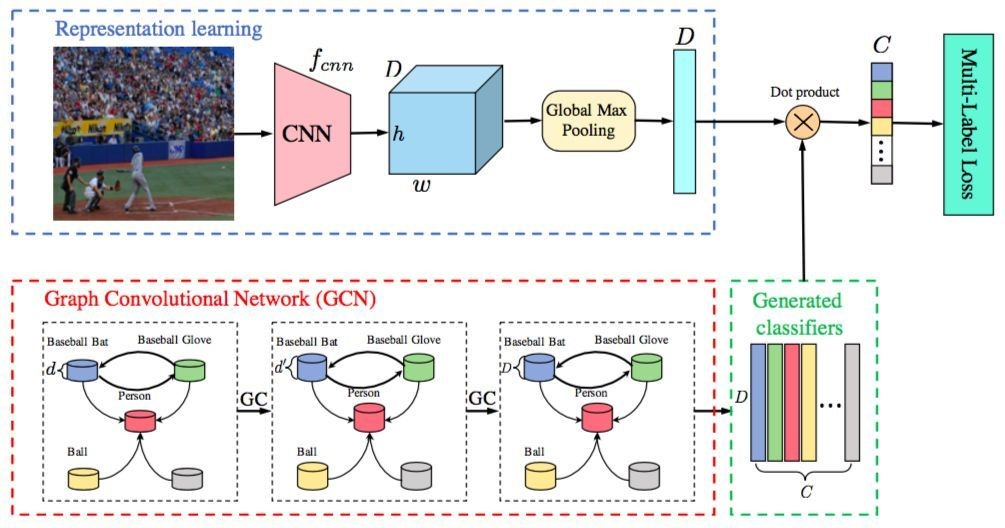
\includegraphics[width=0.75\textwidth]{figures/p3-1.jpg}
	\caption{用于多标签图像识别的 ML-GCN 模型整体框架}\label{fig:simuP1P2Result}
	\vspace{-1em}
\end{figure}

图像特征学习可使用任意基于 CNN的模型学习图像特征。在该的实验中,根据[36,1,15,6],在该实验中使用 ResNet-101 作为实验基础模型;然后应用 全局最大池化 获取图像层面的特征 x :
\begin{equation}
\label{dscNoStgProof0}
x = f_{GMP}(f_{cnn}(I;\theta_{cnn}))\in \mathbb{R}^D
\end{equation}

基于GCN的分类器学习相互依赖的对象分类器,通过基于 GCN 的映射函数从标签特征学习相互依赖的目标分类器$W={w_i}_{i=1}^C$,使用堆叠 GCN,其中每个 GCN 层 I 的输入都取前一层$H^l$的节点特征作为输入,然后输出新的节点特征$H^{l+1}$。第一层的输入是词嵌入向量$Z\in \mathbb{R}^{C\times d}$,矩阵最后一层的输出是分类器$W\in \mathbb{R}^{C\times D}$,通过将所学到的分类器应用于图像特征,得到预测分数:
\begin{equation}
\label{dscNoStgProof0}
\hat{y} = Wx
\end{equation}

假设一张图像的真实标签是 ,那么整个网络可使用传统多标签分类的损失函数来训练,如下:
\begin{equation}
\label{dscNoStgProof0}
loss = \sum_{c=1}^C y^c log(\sigma(\hat{y}^c))+(1-y^c)log(1-\sigma(\hat{y}^c))
\end{equation}

\section{ML-GCN的相关矩阵}
GCN的工作原理是基于相关矩阵在节点间传播信息。所以在GCN中,一个至关重要的问题就是我们如何建立相关矩阵A。在大多数应用中,相关矩阵是预先定义的,但是在目前我们所使用的这些标准多标签图像识别数据集中都没有被提供。本文采用数据驱动的方法建立了相关矩阵。换就话说我们定义标签之间的相关性方式是通过挖掘标签在数据集中的共现模式来实现的。
我们以条件概率的形式对标签相关性依赖关系进行建模,即用$P(L_j|L_i)$表示当标签$L_i$出现时,标签$L_j$出现的概率。 如图9当“冲浪板”时,“人”也会以很高的概率出现,然而,在“人”出现的情况下,“冲浪板”不一定会出现,因此$P(L_j|L_i)$不等于$P(L_i|L_j)$,所以相关系数矩阵不是对称的。

\begin{figure}[htbp!]
	\centering
	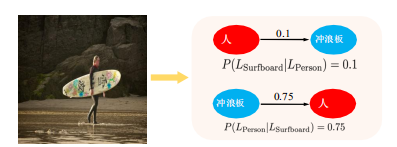
\includegraphics[width=0.75\textwidth]{figures/p3-2.png}
	\caption{图9}\label{fig:pic9}
	\vspace{-1em}
\end{figure}


在构造相关矩阵时,首先计算训练集中标签对的出现次数,得到矩阵$M\in \mathbb{R}^{c\times b}$,具体地说,$C$是类别数,$M_{ij}$表示$L_i$和$L_j$的并发次数。然后,利用这个标记共现矩阵,我们可以通过:
\begin{equation}
\label{dscNoStgProof0}
P_i = \frac{M_i}{N_i}
\end{equation}

6式中,$N_i$表示$L_i$在训练集中的出现次数,$P_{ij}=P(L_j|L_i)$表示$L_i$出现时标签$L_j$的概率。但是6式中简单的相关性或许存在两个缺点。第一,标签和其他标签之间的共现模式可能表现出长尾分布,且可能存在噪声等部分极其不常见的共现。第二,绝对共现次数在训练和测试两个反面可能存在差异。训练集的相关矩阵过拟合会影响泛化能力。因此,我们建议对相关$P$进行二值化。具体地说,我们使
\begin{equation}
A_{ij} =\left\{
\begin{array}{lr}
0, & P_{ij}\textless \tau, \\
1, & P_{ij}\geq \tau. \\
\end{array}
\right. 
\label{con:Gamma_n}
\end{equation}

用阈值$\tau$ 来滤除噪声边缘,其运算可以写成:阵:

根据(2)式得到的过度平滑问题,我们可以得出:当在GCN之后,节点的特征将由自身特征和相邻节点特征的加权和得到。其次,二元相关矩阵存在一个直接问题就是会导致过度平滑。换句话说,由于节点特征可能被过度平滑,导致来自不同簇的节点可能变得难以区分\cite{Jiang2016CNN}。为了缓解这一问题,提出了以下重加权方案:
\begin{equation}
A'_{ij} =\left\{
\begin{array}{lr}
\frac{p}{\sum_{j=1,i\neq j}^C A_{ij}}, & i\neq j, \\
1-p, & i=j. \\
\end{array}
\right. 
\label{con:Gamma_n}
\end{equation}

在上8式中$A'_{ij}$是重新加权的相关矩阵,分配给节点本身和其他相关节点的权重由$p$确定。当节点更新节点特征时,通过这种方式可以使节点本身的权重固定,从而其相关节点的权重便由邻域分布决定。当$p->1$、不考虑节点本身的特性。而另一方面,当$p->0$,相邻信息往往被忽略。


\chapter{实验验证与结果分析}
在本节中,我们首先描述评估指标、数据集和实现细节。然后,我们报告在MS-COCO\cite{Jiang2016CNN}和VOC 2007\cite{Zhang2007ML}了两个多标签图像识别数据集的实验验证结果。最后通过消融实验进行验证。

\section{评价指标}
按照常规设置[28,6,36],按照常规设置[28,6,36],我们分别评估了以下几种指标,其中分别包括查全率OR、总体的查准率OP 和 OF1以及分别在每个类的查准率CP,查全率 CR和CF1。其计算方式如下:

\begin{figure}[htbp!]
	\centering
	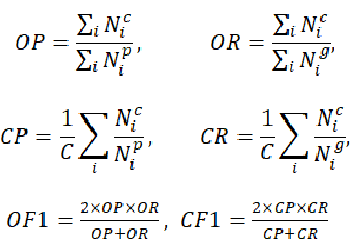
\includegraphics[width=6cm, height=4cm]{figures/123.png}
	%\caption{}\label{fig:123}
	\vspace{-1em}
\end{figure}

对于每个图像,如果它们的置信度大于0.5,则预测标签为正。为了进行公平的比较,我们还报告了前3名的标签的结果cf.[36,6]。此外,我们还计算并报告了平均精度(mAP)。mAP作为通用的对于多标签图像分类方法的评价标准,即平均精度AP和平均精度均值mAP, 对于每一个类,我们将该类在模型中的预测分数,按照降序排列所有的测试样本。在此后,第i个类的平均精度AP被定义为
\begin{equation}
\label{dscNoStgProof0}
AP_i = \frac{\sum_{k=1}^{p}P_i(k)rel_i(k)}{\sum_{k=1}^{R}rel_i(k)}
\end{equation}

$R$代表着测试样本的总数量;如果在第$k$个位置,测试样本是属于第i个类别的,那么$rel(k)=1$,否则$rel(k)=0$。$P(k)$是在第$k$个位置的精确度将其定义为
\begin{equation}
\label{dscNoStgProof0}
P_i(K) = \frac{\sum_{i=1}^{K}rel_i(k)}{K}
\end{equation}

最后,通过在所有类别上对AP取平均数得到mAP作为评估指标。一般而言,总体平均OF1、平均每级CF1和mAP对于性能评估相对更重要。

\section{数据集}

\subsection{MS-COCO数据集}
MS-COCO\cite{Jiang2016CNN}是一个普遍用于多标签图像识别的数据集。该数据集被分为训练集和数据集,其训练集中含有82,081张图,验证集中有40504张图像。这些对象被分为80个类,每个图像大约有2.9个对象标签。COCO数据集中存在很多背景非常复杂目标图像,而且有些图像所包含的目标非常多,有的图片更甚至包含最多达18个标签,同时COCO 数据集还普遍存在的一个问题就是图片的目标特别小,哪怕是人,在不仔细观察的情况下,也很难发现,这些问题这使得多标签图像识别模型在MS-COCO数据集上更具挑战性。

\subsection{PASCAL VOC2007数据集}
PASCAL VOC2007是另一个用于多标签识别的流行数据集。VOC2007数据集同样被分为训练集和测试机集,其中测试集中图片数量约为4952张,训练集则有5011张图片,这9963幅图片总共来自20个对象类别的。在PASCAL VOC2007数据集中,每个图像中的目标都被标有类型信息和坐标信息,所以通过处理PASCAL VOC2007数据集中的标签,就很容易的将其变成多标签图像分类的数据集,该数据集也被很多研究者用来评估多标签图像模型的分类性能。

\section{实验过程}

ML-GCN由两个输出维度分别为1024和2048的GCN层组成。对于标签表示,我们采用了在维基百科数据集上训练过的300维手套\cite{Xue2011Correlative}。对于名称包含多个单词的类别,我们获得了所有单词嵌入的平均值作为标签表示。对于相关矩阵,我们将式(7)中的$\tau$设为0.4,式(8)中的p设为0.2。在图像表示学习分支中,采用负斜率为0.2的LeakyReLU作为非线性激活函数,在实验中收敛速度较快。我们采用ResNet-101\cite{Read2008Multi}作为特征提取骨干,在ImageNet\cite{Tsoumakas2007Random}上进行预训练。在训练过程中,输入图像被随机裁剪并调整大小为448×448,并随机水平翻转以增加数据。对于网络优化,SGD被用作优化器。动量设为0.9。重量衰减为104。每40个学习阶段衰减10倍并且刚开始学习率为0.01,该网络共被训练100个学习阶段。我们实现了基于PyTorch的网络

\section{实验结果展示和分析}
实验中比较了当前主流的的方法了,有CNN-RNN\cite{Jiang2016CNN}、RNN-Attention、Order-Free-RNN\cite{Chen2017Order}、ML-ZSL\cite{Li2015Leveraging}、SRN[36]、Multi-Evidence\cite{Clare2002Knowledge}等最新研究方法,给出了基于二元相关矩阵(ML-GCN(binary))和重加权相关矩阵(ML-GCN(re-weighted))的结果。显而易见,我们基于二元相关矩阵的ML-GCN方法获得了较差的分类性能,这可能主要是由于我们上一章节讨论的过度平滑问题。所提出的重加权方案可以缓解过平滑问题,从而获得更优的性能。与目前最新的方法相比,我们提出的重加权方案在几乎所有指标下都表现得更好,这表明了我们提出的ML-GCN及其相应的重加权方案的有效性。表1是在MS-COCO数据集上的与几种新方法的比较。报告了基于两种相关矩阵的ML-GCN的性能。“二元”表示我们使用二元相关矩阵(7)。“重加权”表示使用所提出的重加权方案产生的相关矩阵。表2表示的是在VOC 2007数据集上,ML-GCN与目前知名的多标签图像分类的方法的AP和mAP比较情况。“二进制”和“重新加权”的含义与表1相同。

\begin{figure}[htbp!]
	\centering
	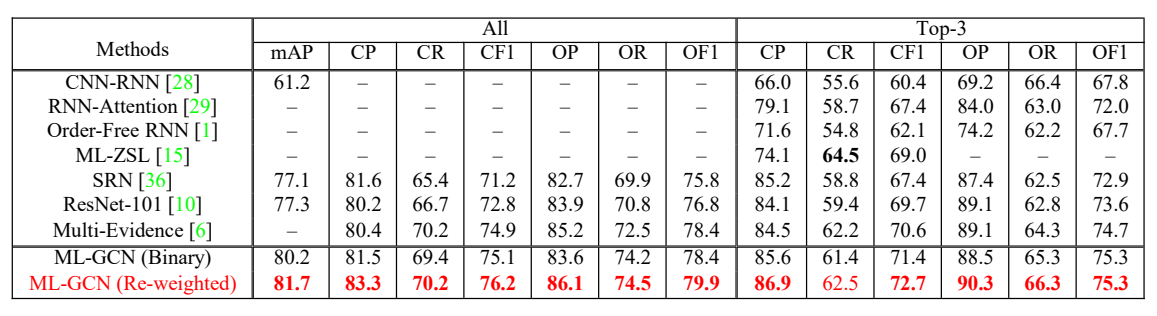
\includegraphics[width=14cm, height=5cm]{figures/p4-1.png}
	\caption{COCO数据集中的结果}\label{fig:p4-1}
	\vspace{-1em}
\end{figure}

\begin{figure}[htbp!]
	\centering
	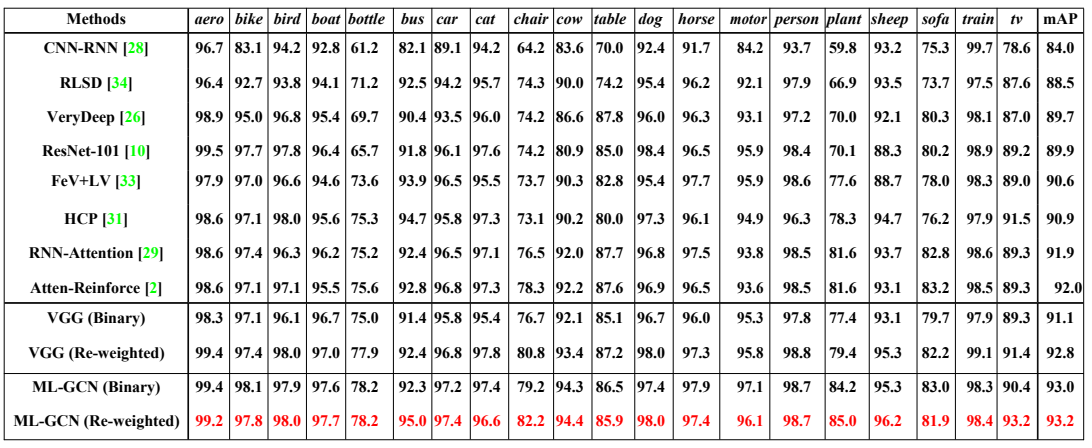
\includegraphics[width=14cm, height=6cm]{figures/p4-2.png}
	\caption{VOC 2007数据集中结果}\label{fig:p4-2}
	\vspace{-1em}
\end{figure}

由于之前很多关于VOC 2007数据集的研究都是基于VGG模型的\cite{Li2014Multi}。为了公平比较,我们还报告了使用VGG模型作为基础模型的结果。显然,通过数据对比,可以发现我们所介绍ML-GCN的方法比目前主流的方法有了明显的改进。具体地说,采用我们的重加权方案的ML-GCN得到93.2\%的mAP,其性能比目前最先进的方法高出\%2。即使使用VGG模型作为基础模型,我们仍然可以获得更好的结果(+0.4\%)。此外,与MS-COCO的结果一致,在VOC上重新加权的方案比二元相关矩阵也有更好的性能。

\section{消融研究}
在本节中,我们从四个不同的方面进行消融研究,包括ML-GCN对不同类型的词嵌入的敏感性、$\tau$对相关矩阵二值化的影响、p对相关矩阵重加权的影响以及GCN的深度。

\subsection{不同阈值$\tau$的影响}

我们研究了不同阈值$\tau$的影响。对于相关矩阵二值化,我们在第三章等式(7)中改变阈值$\tau$的值,并在图10中显示结果。注意,如果我们不过滤任何边,模型就不会收敛。因此,该图中没有$\tau=0$的结果。正如图10所示,在滤除噪声边缘,使得多标签识别的精度精度提高。然而,当过多的边缘被过滤掉时,由于相关的邻域也会被忽略,所以精度会下降。MS-COCO和VOC 2007的$\tau$的最佳值均为0.4

\begin{figure}[htbp]
	\centering
	\subfigure[在COCO数据集中]{
		\begin{minipage}[t]{0.5\linewidth}
			\centering
			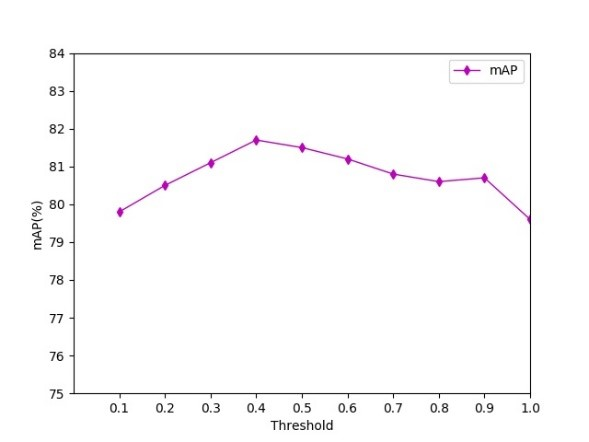
\includegraphics[width=7cm, height=6cm]{figures/p4-3a.jpg}
			%\caption{fig1}
		\end{minipage}%
	}%
	\subfigure[在VOC数据集中比]{
		\begin{minipage}[t]{0.5\linewidth}
			\centering
			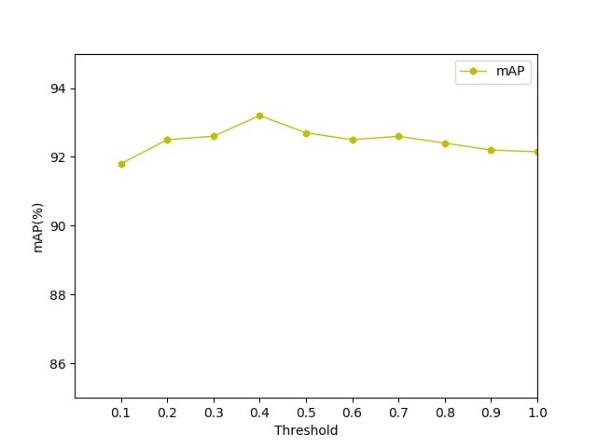
\includegraphics[width=7cm, height=6cm]{figures/p4-3b.jpg}
			%\caption{fig2}
		\end{minipage}%
	}%
	 
	\centering
	\caption{不同T值精度比较}
\end{figure}


\subsection{不同p对相关矩阵重加权的影响}
不同p对相关矩阵重加权的影响为了探讨第三章公式(8)中p的不同值对多标签分类精度的影响,我们改变了{0,0.1,0.2,…,0.9,1}中p的值,如图11所示。一般来说,此图显示在更新GCN中的节点特征时,平衡节点本身和邻域之间的权重的重要性。在实验中,我们通过交叉验证来选择p的最优值。我们可以看到,当p=0.2时,它在MS-COCO和VOC 2007上都能达到最佳性能。如果p太小,则图的节点(标签)无法从相关节点(标签)获得足够的信息。而如果p值太大,则会导致过度平滑。


\begin{figure}[htbp]
	\centering
	\subfigure[在COCO数据集中]{
		\begin{minipage}[t]{0.5\linewidth}
			\centering
			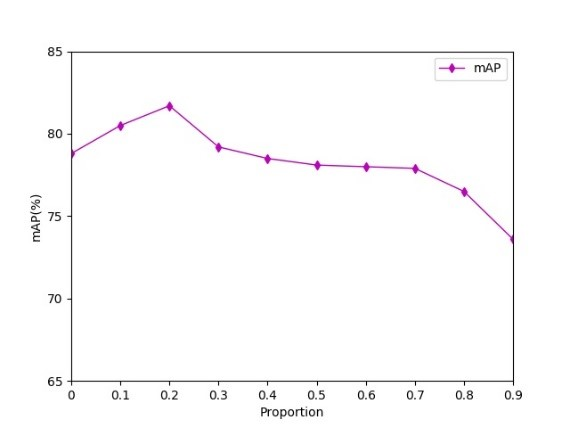
\includegraphics[width=7cm, height=6cm]{figures/p4-4a.jpg}
			%\caption{fig1}
		\end{minipage}%
	}%
	\subfigure[在VOC数据集中比]{
		\begin{minipage}[t]{0.5\linewidth}
			\centering
			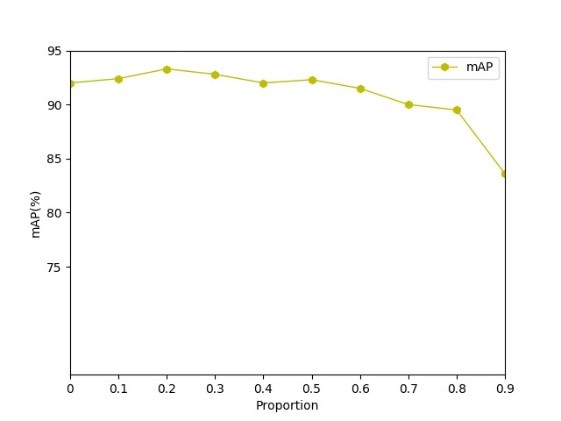
\includegraphics[width=7cm, height=6cm]{figures/p4-4b.jpg}
			%\caption{fig2}
		\end{minipage}%
	}%
	\centering
	\caption{不同p值精度比较}
\end{figure}

另一个有趣的观察是,当p=0时,我们可以得到MS-COCO上81:67\%和VOC 2007上93:15\%的映射,这仍然优于现有的方法。注意,当p=0时,我们本质上没有显式地合并标签相关性。改进得益于我们的ML-GCN模型通过共享的基于GCN的映射函数从先前的标签表示中学习对象分类器,该映射函数隐式地对标签依赖关系建模.

对于卷积层数是否越深越好本实验也做了探究,我们在表6中显示了我们的
\begin{figure}[htbp!]
	\centering
	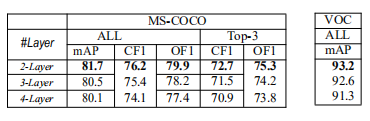
\includegraphics[width=0.75\textwidth]{figures/p4-5.png}
	\caption{卷积层深度影响}\label{fig:p4-5}
	\vspace{-1em}
\end{figure}

模型在不同数量的GCN层下的性能结果。对于三层模型,连续层的输出维数分别为1024、1024和2048。对于四层模型,维度为1024、1024、1024和2048。如图所示,当图卷积层数增加时,两个数据集上的多标签识别性能下降。性能下降的可能原因是,当使用更多的GCN层时,节点之间的传播将累积,这可能导致过度平滑。

\subsection{不同类型的词嵌入方式影响}
\begin{figure}[htbp!]
	\centering
	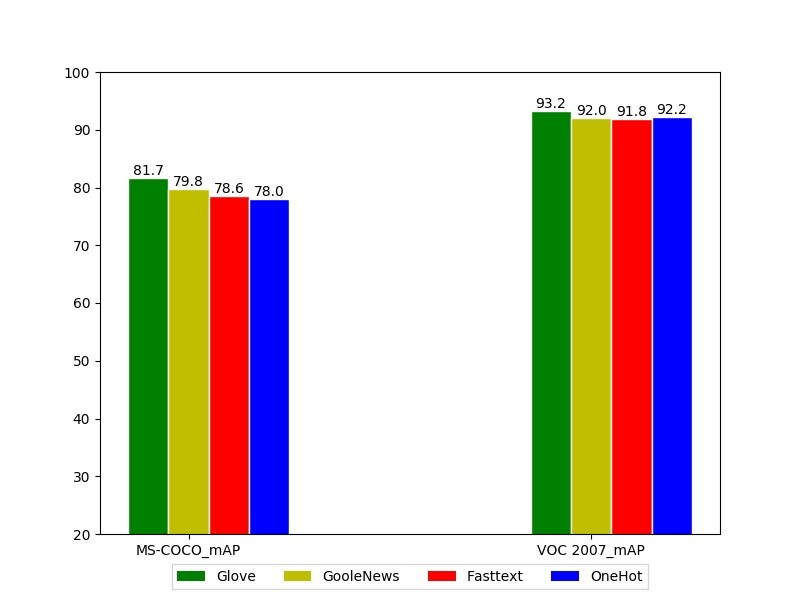
\includegraphics[width=0.75\textwidth]{figures/p4-6.jpg}
	\caption{不同字嵌入方法的对比}\label{fig:simuP1P2Result}
	\vspace{-1em}
\end{figure}
ML-GCN在不同类型的词嵌入下,该实验使用Glove\cite{Xue2011Correlative}作为标签表示,它作为堆叠GCN的输入,用于学习对象分类器。在这一部分中,我们评估了ML-GCN在其他类型的流行词汇表示下的性能。具体来说,我们研究了四种不同的单词嵌入方法,包括GloVe\cite{Xue2011Correlative}、GoogleNews\cite{Guo2011Multi}、FastText和simple-one-hot-word嵌入。图12显示了在MS-COCO和VOC 2007上使用不同单词嵌入的结果。如图所示,当使用不同的词嵌入作为GCN的输入时,多标签识别精度不会受到显著影响。此外,观察结果(尤其是一个hot的结果)证明,ML-GCN方法所获得的准确性改进并非完全来自于单词嵌入所产生的语义。此外,使用强大的单词嵌入可以带来更好的性能。对于语义相关的概念,它们的嵌入在嵌入空间中是紧密的。我们的模型可以利用这些隐含的依赖关系,进一步有利于多标签图像识别。



\chapter{总结与展望}

\section{总结}

在目前计算机视觉领域中具有挑战性研究中,多标签图像分类便是其中之一。在目前的信息大爆炸时代,互联网尤其是移动互联网每天都在产生海量的图像数据,这些图像中包含了重要的有价值的数据,为了更方便的获的图片中有价值的信息,对这些图片进行分类显得尤为重要。现如今在在人脸识别、图片搜索以及农业、医疗、工业甚至军事领域都有普遍使用多标签图像分类技术,这充分展现了多标签分类技术的重要研究意义和价值。我们在这篇文章中对多标签分类技术以及其在多标签图像分类中的方法进行了部分探究,本文的主要工作总结如下:
1.首先我们对多标签分类技术及其在多标签图像分类中方法的研究意义、背景以及国内外现状进行了系统的概述和分析,同时从基于问题转化和算法自适应两个方面介绍了相关方法和理论,其次我们还简要介绍多标签图像分类的评价指标,分析了部分算法的优缺点。
2.由于在多标签图像中,目标特征存在很多相互关联性的特点,所以在这篇文章中我们尝试并且通过实验验证基于图卷积卷积神经网络(ML-GCN)的方法,在这种多标签图像分类模型中使用图结构对标签之间的相关性进行建模。系统的阐述了基于GCN的模型,从已有的标签表示中学习依赖对象的分类器。为了显式地建立标签依赖关系模型,我们设计了一种新的加权模式,通过平衡节点与其八个节点之间的权值来构造GCN的相关矩阵。通过实验验证,我们得出这种方案有效地缓解影响GCN性能的两个主要因素:过拟合和过平滑。

\section{展望}
本文中ML-GCN方法中GCN上面CNN这两个分支是独立的,将CNN里面的图像特征运用到GCN的学习过程中是否有待改进,通过改进分类效果可否更好。其次,分类器本质上就是一个分类超平面吧,给定特征图,通过反向传播,对全连接层训练得到的超平面理论上已经是能把训练集上的样本区分的最好了.是否可以通过运用全连接层训练构建超平面得到更好的效果。


